\section{The \ara{} Compiler}
\label{sec:ingestor}

The born-agent pathway (\S\ref{sec:live-pm}) produces the highest-fidelity \ara{}s by capturing knowledge as it emerges during the research process.
However, the scientific record contains millions of legacy PDFs that were never structured, and the born-agent pathway cannot reach backward.
Beyond the PDF itself, research knowledge is distributed across complementary sources: GitHub repositories encode implementation decisions that prose omits, expert-curated evaluation rubrics encode what domain practitioners consider the core claims, and recorded experimental trajectories preserve the failure modes that papers systematically suppress.
To bridge this gap, we introduce the \textbf{\ara{} Compiler}, an agent skill that translates any combination of legacy research sources into a complete \ara{}.\footnote{\url{github.com/AmberLJC/Agent-Native-Research-Artifact}}
Quality is enforced in two stages. During compilation, the Compiler uses only ARA Seal Level~1 as an in-loop validation signal. After compilation, the finished artifact enters the downstream Seal pipeline, where Levels~2--3 evaluate its argumentative support and empirical reproducibility (\S\ref{sec:liveness}).

\begin{figure}[!t]
    \centering
    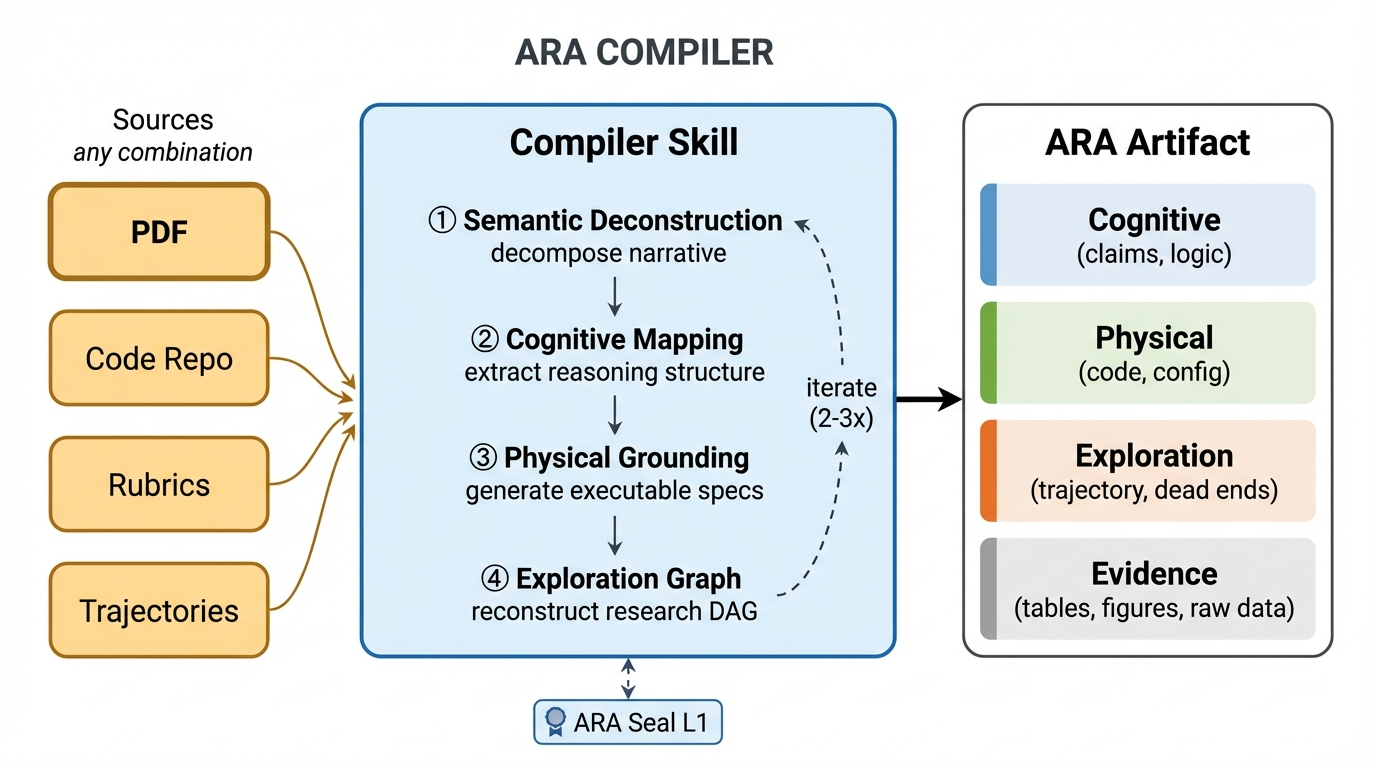
\includegraphics[width=\linewidth]{figures/fig_compiler_v2.png}
    \caption{The \ara{} Compiler accepts any combination of research sources and guides a coding agent through four stages of top-down artifact compilation, iterating 2--3$\times$ with in-loop ARA Seal Level~1 validation until the output conforms to the protocol.}
    \label{fig:ingestor-pipeline}
    \end{figure}
    
\subsection{Design Principles}
\label{sec:ingestor-principles}

\paragraph{Universal input, canonical output.}
The Compiler is many-to-one: it accepts any combination of PDFs, code repositories, datasets, human-curated rubrics (e.g., PaperBench~\citep{starace2025paperbench} claim decompositions), and experimental trajectory logs (e.g., RE-Bench~\citep{wijk2025rebench} traces that record failures the paper omits), and always produces a single \ara{} conforming to \S\ref{sec:protocol}.
Degradation is graceful: a PDF alone yields a valid artifact with stub-level physical layers; richer inputs populate progressively more complete layers.

\paragraph{High-fidelity preservation.}
A narrative paper compresses and selects; the Compiler decompresses and restores.
Every numerical result, hyperparameter, architectural detail, and negative finding in the sources must appear \emph{somewhere} in the artifact, and any PDF-accessible information missing from the \ara{} constitutes a compilation failure (evaluated in \S\ref{sec:eval-understanding}).
Preservation is faithful to sources; \emph{enrichment} (\S\ref{sec:collective}) separately surfaces cross-artifact patterns no single source expresses.

\paragraph{Knowledge lineage, not flat extraction.}
Narrative compilation destroys the \emph{provenance chains} connecting claims to experiments, experiments to evidence, and evidence to code.
Plain-text extraction recovers content but not these connections: parsing a PDF into Markdown populates four directories yet leaves them structurally isolated.
The Compiler performs \emph{forensic reconstruction}, recovering the cross-layer forensic bindings (\S\ref{sec:layers}) from sources where lineage exists only implicitly---scattered across prose, figure captions, appendix tables, and code comments---so an agent can trace any claim downstream to code or any number upstream to its hypothesis.
Recovering this lineage, not populating layers, is the core compilation problem.

\subsection{Compiler Implementation}
\label{sec:ingestion-skill}

Realizing these principles against narrative PDFs requires concrete mechanisms that address the specific ways prose obscures structure, lineage, and source diversity.
The Compiler is implemented as a single agent skill (Figure~\ref{fig:ingestor-pipeline}) that guides a coding agent through the translation from legacy sources to \ara{} format.
The skill prompt encodes the full \ara{} schema, field-level requirements, and a structured generation protocol.
We describe the key elements below; the complete skill specification is reproduced in Appendix~\ref{app:ingestor-prompt}.

\paragraph{Top-down generation.}
The skill instructs the agent to construct the artifact \emph{top-down}, mirroring how a researcher explains their work to a new collaborator: high-level concepts first, details next, implementation last.
Concretely, the agent proceeds through four stages.
\emph{Semantic Deconstruction} strips narrative framing to expose raw research content (formulations, configurations, results, dependencies, failed approaches), rewritten in fact-dense telegraphic form that eliminates the Storytelling Tax at the source level.
\emph{Cognitive Mapping} populates \texttt{/logic}: motivation chain (observations $\to$ gaps $\to$ insight), falsifiable claims with proof pointers, formal concepts, and the solution structure, with every claim linked to the experiment that verifies it.
\emph{Physical Grounding} generates \texttt{/src}: annotated configurations, typed code stubs, and the environment manifest; when a code repository is available, stubs are replaced with actual implementations and the agent performs \emph{code-paper reconciliation}, cross-referencing the codebase against claims to surface tacit knowledge---implicit assumptions, undocumented tricks, extra parameters~\citep{li2026tacit}---that is written back to \texttt{/logic} as provenance-tagged heuristics.
\emph{Exploration Graph Extraction} reconstructs the research DAG as a nested YAML tree with dead-end leaf nodes documenting hypothesis, failure mode, and lesson.
This ordering ensures each layer is informed by the one above: cognitive structure guides physical generation, and the exploration graph contextualizes both.

\paragraph{Iterative refinement via validation feedback.}
After initial generation, ARA Seal Level~1 checks (\S\ref{sec:liveness})---schema conformance, cross-layer reference resolution, required field completeness---run within the same agent conversation, returning failures as structured diagnostics that drive targeted fixes.
This generate\,$\to$\,validate\,$\to$\,fix loop typically converges in 2--3 rounds, turning Level~1 into actionable feedback rather than a post-hoc report.

\paragraph{Source-aware enrichment.}
\label{sec:collective}
Auxiliary sources are routed to the layer they most directly populate: code repositories replace stubs with verified implementations in \texttt{/src}; evaluation rubrics anchor \texttt{/logic} with expert-verified claim decompositions; and trajectory logs seed \texttt{/trace} with dead-end nodes the PDF omits.
When a library of previously compiled \ara{}s is available, the Compiler further performs \emph{collective inference}: it retrieves heuristics and configurations from same-domain artifacts, flags common patterns the current paper omits, and adds them as candidate heuristics tagged \texttt{collective\_inference} so downstream agents can distinguish stated from inferred knowledge.
